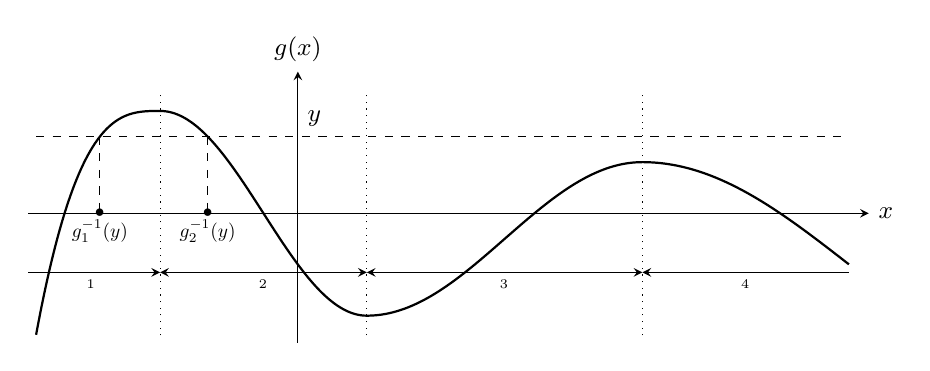
\begin{tikzpicture}%[scale=.9]
\shorthandoff{>}
%
\pgfmathsetmacro{\sx}{1.75};% x-scaling
%
% transformacion g' = 0 medida nula
\begin{scope}
%
\pgfmathsetmacro{\sy}{1.3};% y-scaling 
%
\draw[>=stealth,->] ({-1.9*\sx-.1},0)--({\sx*4+.25},0) node[right]{\small $x$};
\draw[>=stealth,->] (0,{\sy*(-3*.9^3+1)-.1})--(0,{\sy+.5}) node[above]{\small $g(x)$};
%
\draw[thick]
plot[domain=-1.9:-1,samples=100] ({\sx*\x},{\sy*(3*(\x+1)^3+1)})
-- plot[domain=-1:.5,samples=100] ({\sx*\x},{\sy*cos(120*(\x+1))})
-- plot[domain=.5:2.5,samples=100] ({\sx*\x},{\sy*(.75*sin(90*(\x-1.5))-.25)})
-- plot[domain=2.5:4,samples=100] ({\sx*\x},{\sy*(cos(60*(\x-2.5))-.5)})
;
%
\draw[dashed] ({-1.9*\sx},{.75*\sy})--({4*\sx},{.75*\sy});
\draw (0,{.75*\sy}) node[above right]{\small $y$};
%
\draw[dashed] ({-\sx*(1+(.25/3)^(1/3))},{.75*\sy})--({-\sx*(1+(.25/3)^(1/3))},0)
node[scale=.7]{$\bullet$} node[below,scale=.7]{$g_1^{-1}(y)$};
%
\draw[dashed] ({\sx*(acos(.75)/120-1)},{.75*\sy})--({\sx*(acos(.75)/120-1)},0)
node[scale=.7]{$\bullet$} node[below,scale=.7]{$g_2^{-1}(y)$};
%
%
\draw[dotted] ({-\sx},{-\sy-.25})--({-\sx},{\sy+.25});
\draw[>=stealth,->] ({-\sx*1.9-.1},-.75)--({-\sx},-.75);
\draw ({-1.5*\sx},-.75) node[below,scale=.8]{\small $\X_1$};
%
\draw[dotted] ({.5*\sx},{-\sy-.25})--({.5*\sx},{\sy+.25});
\draw[>=stealth,<->] ({-\sx},-.75)--({.5*\sx},-.75);
\draw ({-.25*\sx},-.75) node[below,scale=.8]{\small $\X_2$};
%
\draw[dotted] ({2.5*\sx},{-\sy-.25})--({2.5*\sx},{\sy+.25});
\draw[>=stealth,<->] ({.5*\sx},-.75)--({2.5*\sx},-.75);
\draw ({1.5*\sx},-.75) node[below,scale=.8]{\small $\X_3$};
%
\draw[>=stealth,<-] ({2.5*\sx},-.75)--({4*\sx},-.75);
\draw ({3.25*\sx},-.75) node[below,scale=.8]{\small $\X_4$};
\end{scope}
%
%
% % reparticion
% \begin{scope}[xshift=8.5cm]
% %
% \pgfmathsetmacro{\sy}{2};% y-scaling 
% %
% \draw[>=stealth,->] (-.6,0)--({\sx*4+.25},0) node[right]{\small $x$};
% \draw[>=stealth,->] (0,-.25)--(0,{\sy+.5}) node[above]{\small $F_X$};
% %
% \draw[thick] (-.5,0)--(0,0)--(\sx,{\sy/2})--({2*\sx},{\sy/2})
% -- plot[domain=2:3,samples=100] ({\sx*\x},{\sy*(1+(\x-2)^(3/2))/2})
% -- ({\sx*4},\sy);
% %
% \draw (\sx,0)--(\sx,-.1) node[below,scale=.9]{\small $1$};
% \draw ({2*\sx},0)--({2*\sx},-.1) node[below,scale=.9]{\small $2$};
% \draw ({3*\sx},0)--({3*\sx},-.1) node[below,scale=.9]{\small $3$};
% \draw (\sx,0)--(\sx,-.1) node[below,scale=.9]{\small $1$};
% %
% \draw (0,{\sy/2})--(-.1,{\sy/2}) node[left,scale=.7]{\small $1/2$};
% \draw (0,\sy)--(-.1,\sy) node[left,scale=.7]{\small $1$};
% %
% \draw ({\sx*2.25},-1) node{\small (b)};
% \end{scope}
%
\end{tikzpicture}